\documentclass{beamer}

\usepackage{amsmath}
\usepackage{amssymb}
\usepackage{amsthm}
\usepackage{mathtools}
\usepackage[UKenglish]{babel}
\usepackage{enumerate}
\usepackage{graphicx}
\usepackage{braket}
\usepackage{esint}
\usepackage{float}
\usepackage{tabularx}
\usepackage{array}
\usepackage{subcaption}
\usepackage{hyperref}
\hypersetup{colorlinks=false, bookmarks=true}

\usetheme{Madrid}
\usecolortheme{seahorse}
\usefonttheme{professionalfonts}
\useinnertheme{circles}

\AtBeginSection[]
{
  \begin{frame}
    \frametitle{Table of Contents}
    \tableofcontents[currentsection]
  \end{frame}
}

\setbeamertemplate{caption}[numbered]

\title[QCNN State Preparation]{A QCNN for Quantum State Preparation}
\subtitle{Carnegie Vacation Scholarship}
\author[David Amorim]{David Amorim}
\institute[]{}
\date[05/08/2024]{Week 5 \\(29/07/2024 - 02/08/2024)}

\begin{document}

\frame{\titlepage}

\section{Preliminaries}
\begin{frame}
\frametitle{Aims for the Week}
The following aims were set at the last meeting (29/07/2024):

\begin{alertblock}{Improve Loss Function}
Work on an improved version of WILL. Incorporate some phase extraction metrics (e.g. $\chi$, $\epsilon$) into the loss function. 
\end{alertblock}

\begin{alertblock}{Investigate Phase Extraction}
Study the relationship between mismatch and the extracted phase, i.e. study the operator $\tilde{Q}^\dagger (\hat{I} \otimes\hat{R}) \tilde{Q}$. 
\end{alertblock}

\begin{alertblock}{Mitigate Barren Plateaus}
Work on strategies to mitigate barren plateaus, e.g. implement layer-by-layer training.
\end{alertblock}
\end{frame}

\begin{frame}
THIS WEEK INCLUDE EXAMPLES WITH HIGH $m$ !!
\end{frame}

\section{Improving the Loss Function}

\begin{frame}
\frametitle{WILL Revisited}
\begin{itemize}
\item As discussed at the meeting on 29/07, the definition of \alert{WILL} (weighted L$_\text{p}$ loss) was amended to: 
\begin{equation}
\text{WILL}_\text{p,q} =  \left( \sum_k \Big|x_k -y_k \Big|^p \alert{+ |x_k|} \Big|[k]_m - \Psi([k]_n) \Big|^q \right)^{1/p},
\end{equation}
where the changes to the previous definition are highlighted
\item Testing this for different $\Psi$ (with $L=6$, $m=3$ and 600 epochs) yielded the following optimal values for $p$, $q$:
\end{itemize}
\begin{table}
\centering 
\begin{tabular}{c|c| c}
$\Psi(f)$ & $p$ & $q$ \\ \hline 
$\sim f$ & 0.25 & 0.5  \\
$\sim  f^2$ & 1 & 1.5  \\
$\Psi_{\text{H23}}$ & 0.75 & 2  \\
\end{tabular}
\caption{Optimal identified $p$, $q$ values for WILL}
\end{table}
\end{frame}

\begin{frame}
\frametitle{Comparing SAM, WIM, and WILL}
\begin{columns}
\begin{column}{0.5\textwidth}
\begin{table}
\begin{tabular}{c || c| c| c }
& SAM & WIM & WILL \\ \hline \hline 
$\mu$ &  \textbf{3.4e-2} & 6.0e-2 & 4.5e-1 \\
$\sigma$ &  1.4e-1 &1.1e-1 & 4.7e-1 \\
$\epsilon$  &  \textbf{1.9e-2} & 9.2e-2 & 2.6e-1  \\
$\chi$ & \textbf{ 3.2e-2} & 5.1e-2  & 3.7e-1  \\ \hline 
$\Omega$ &  \textbf{4.46} & 3.19 & 0.76
\end{tabular}
\caption{Comparing loss function metrics for $\Psi(f) \sim f$ ($L=6$, $m=3$, 600 epochs)}
\end{table}
\end{column}
\begin{column}{0.5\textwidth}
\begin{figure}
\centering 
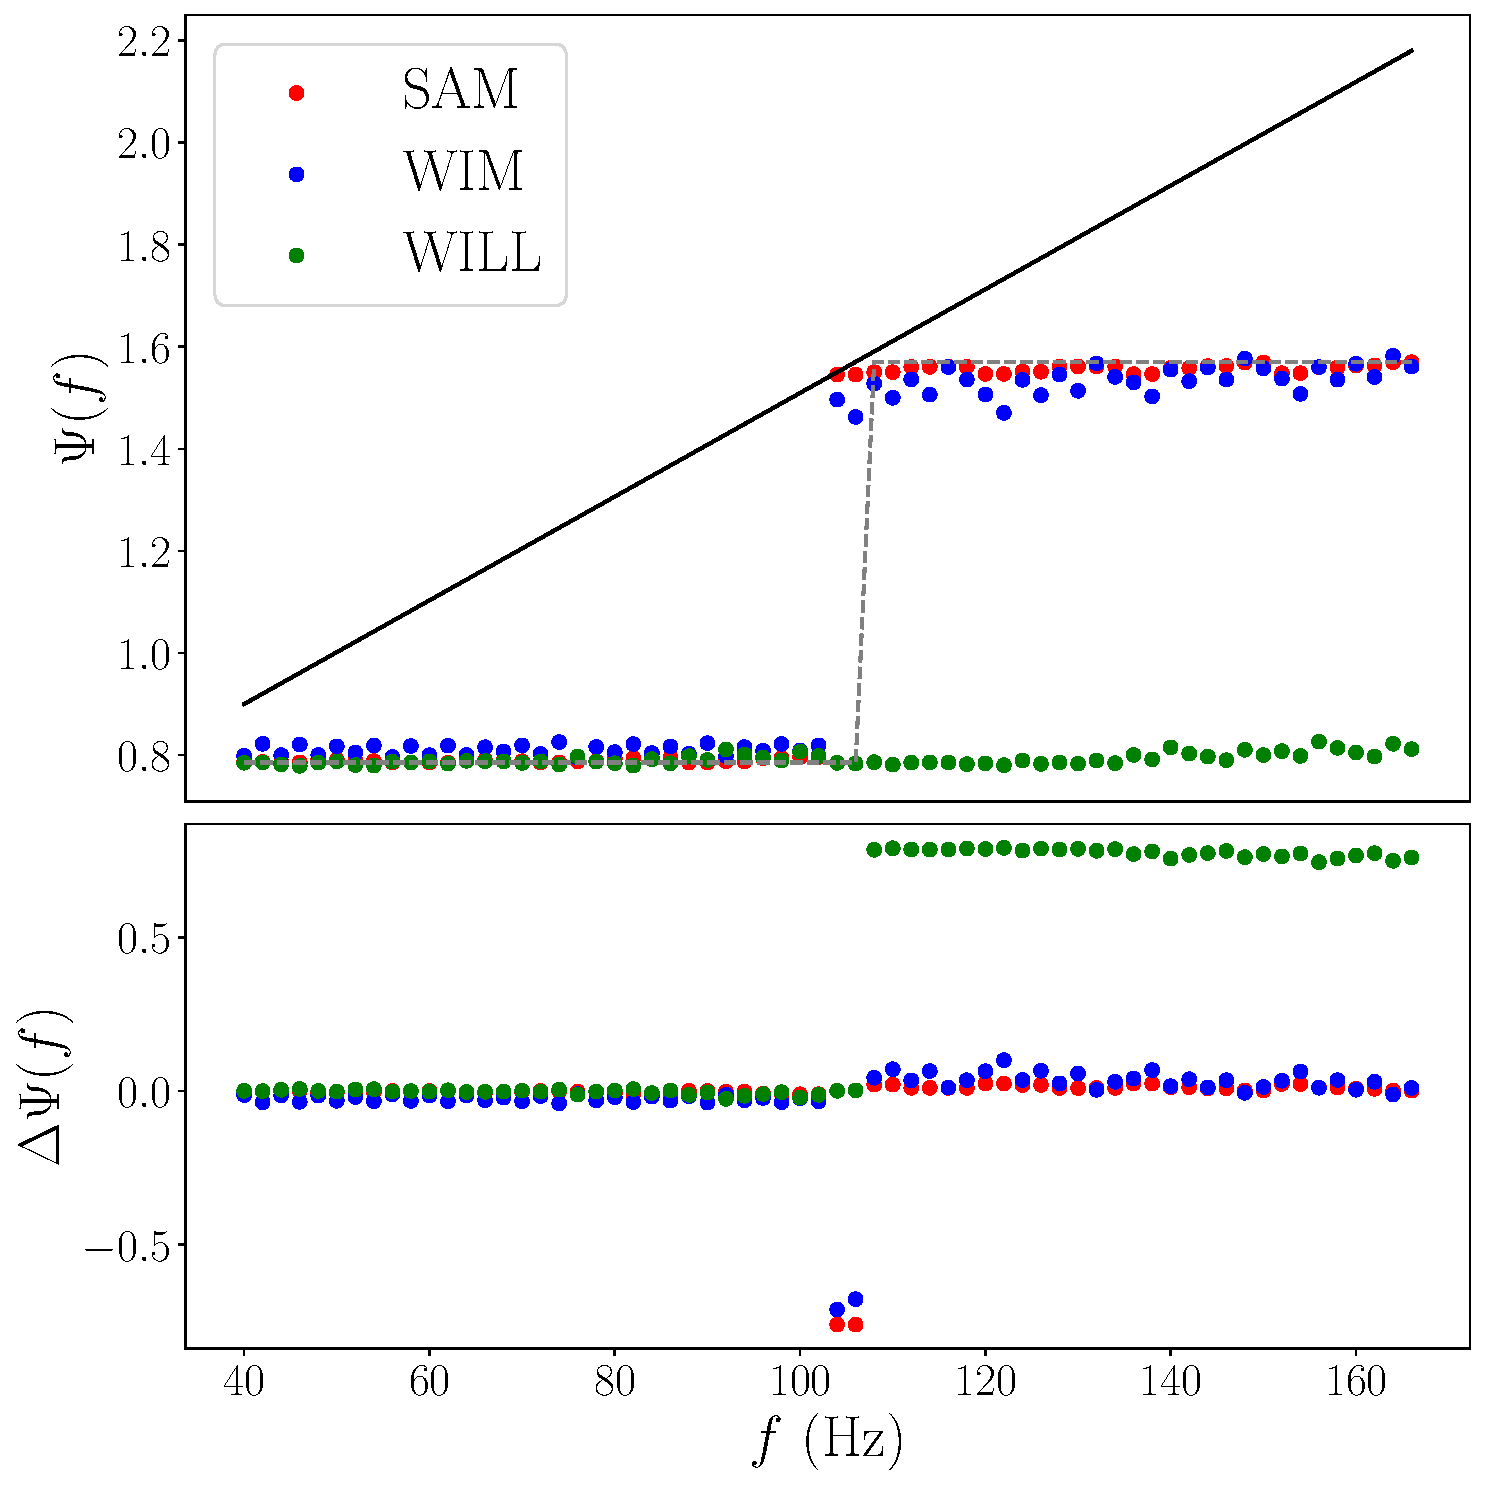
\includegraphics[width=\textwidth]{im/SAM_WIM_WILL_F_new}
\caption{Comparing extracted phase functions for $\Psi(f) \sim f$ ($L=6$, $m=3$, 600 epochs)}
\end{figure}
\end{column}
\end{columns}
\end{frame}

\begin{frame}
\frametitle{Comparing SAM, WIM, and WILL}
\begin{columns}
\begin{column}{0.5\textwidth}
\begin{table}
\begin{tabular}{c || c| c| c }
& SAM & WIM & WILL \\ \hline \hline 
$\mu$ &  \textbf{1.9e-1} & 2.3e-1 & 6.6e-1  \\
$\sigma$ &  1.2e-1 & \textbf{1.0e-1} & 4.1e-1\\
$\epsilon$  &  2.2e-1 & 4.2e-1 & \textbf{2.8e-2}  \\
$\chi$ &  \textbf{1.9e-1} & 2.0e-1 & 6.1e-1  \\ \hline 
$\Omega$ &  \textbf{1.39} & 1.05 & 0.57
\end{tabular}
\caption{Comparing loss function metrics for $\Psi(f) \sim f^2$ ($L=6$, $m=3$, 600 epochs)}
\end{table}
\end{column}
\begin{column}{0.5\textwidth}
\begin{figure}
\centering 
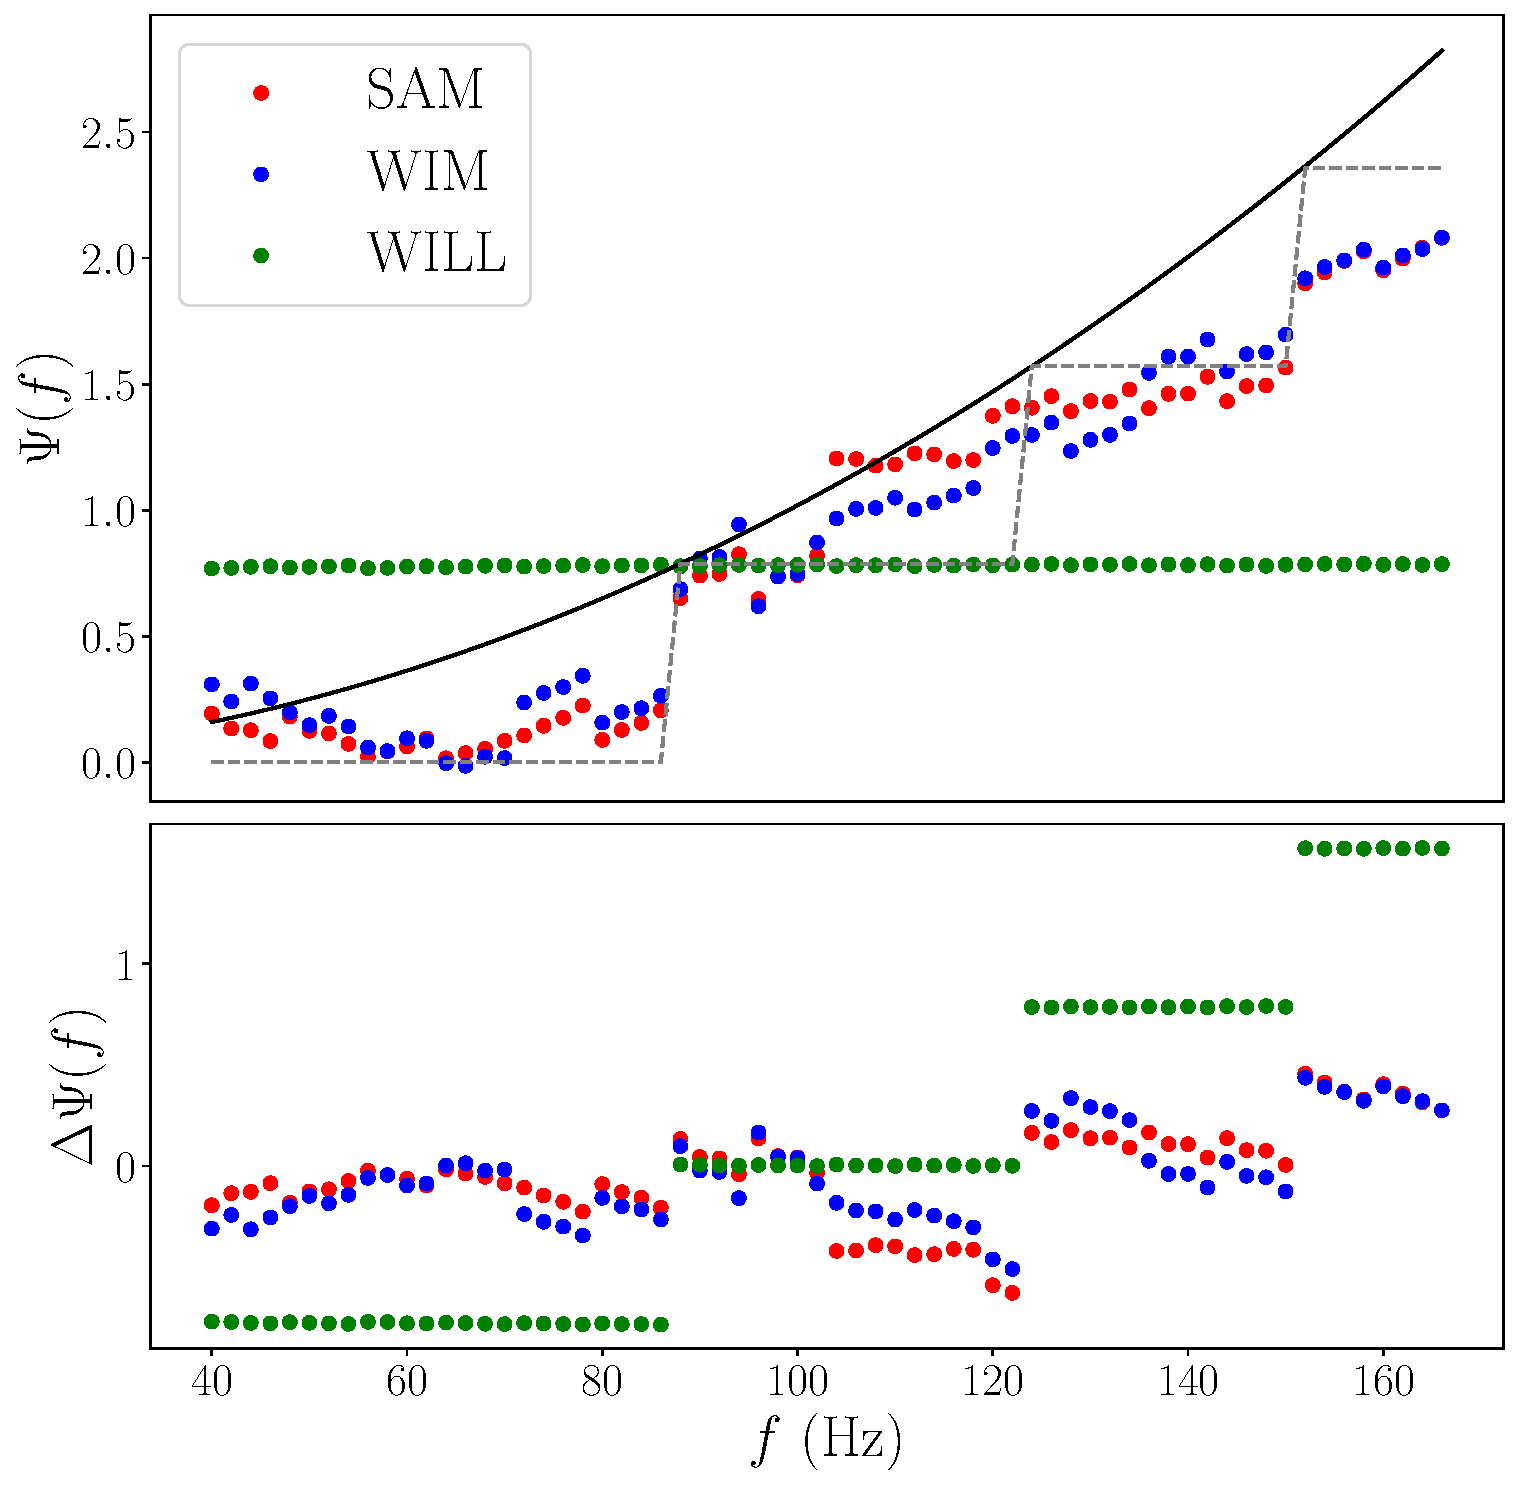
\includegraphics[width=\textwidth]{im/SAM_WIM_WILL_F2_new}
\caption{Comparing extracted phase functions for $\Psi(f) \sim f^2$ ($L=6$, $m=3$, 600 epochs)}
\end{figure}
\end{column}
\end{columns}
\end{frame}

\begin{frame}
\frametitle{Comparing SAM, WIM, and WILL}
\begin{columns}
\begin{column}{0.5\textwidth}
\begin{table}
\begin{tabular}{c || c| c| c }
& SAM & WIM & WILL \\ \hline \hline 
$\mu$ &  \textbf{6.8e-2} & 8.4e-2 & 7.6e-2 \\
$\sigma$ &  1.8e-1 & \textbf{1.2e-1} & 2.6e-1 \\
$\epsilon$  &  4.5e-2 & 1.8e-1 & \textbf{7.3e-3 } \\
$\chi$ &  7.4e-2 & 1.0e-1 & \textbf{6.2e-2} \\ \hline 
$\Omega$ &  \textbf{2.75} & 2.07 & 2.48
\end{tabular}
\caption{Comparing loss function metrics for $\Psi_\text{H23}$ ($L=6$, $m=3$, 600 epochs)}
\end{table}
\end{column}
\begin{column}{0.5\textwidth}
\begin{figure}
\centering 
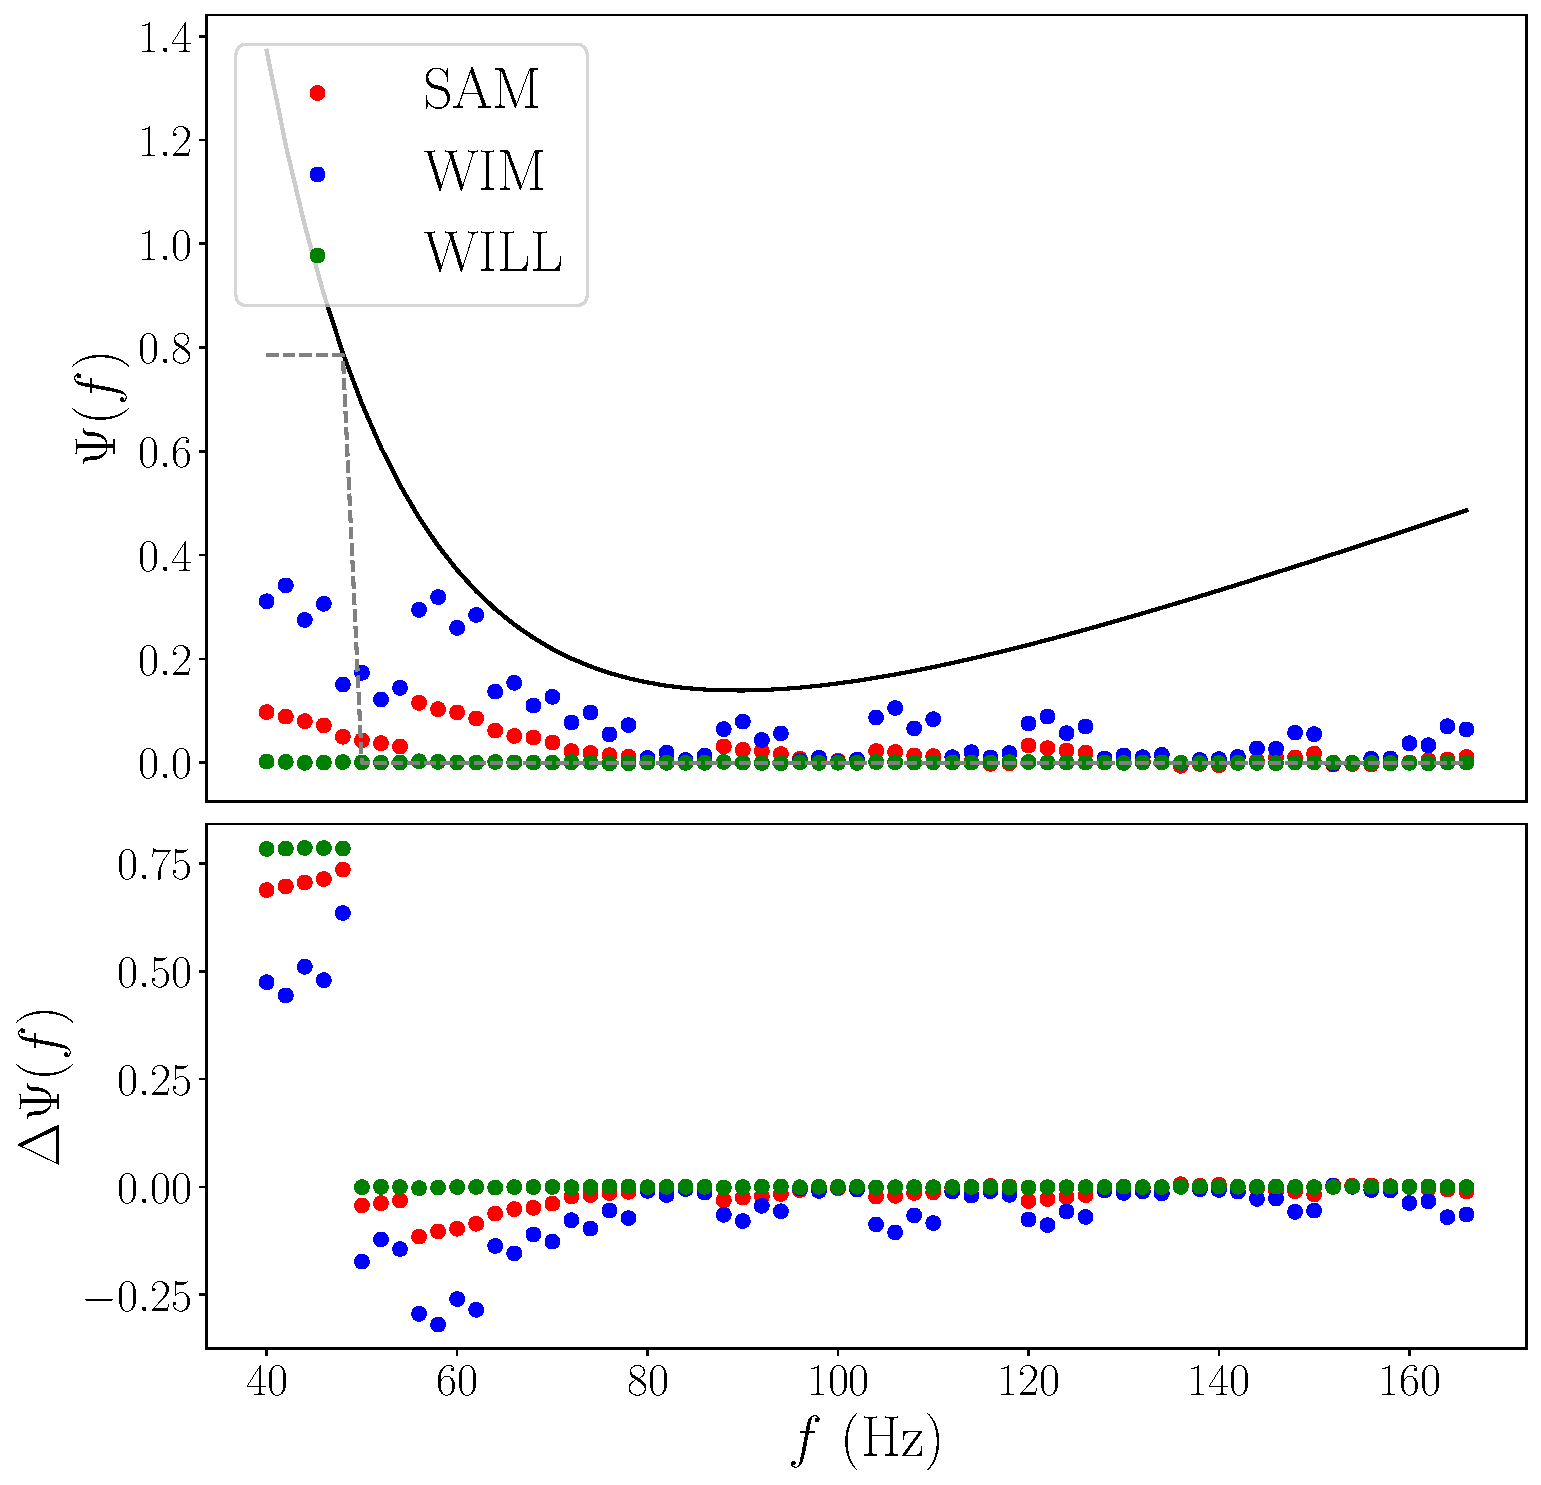
\includegraphics[width=\textwidth]{im/SAM_WIM_WILL_H_new}
\caption{Comparing extracted phase functions for $\Psi_\text{H23}$ ($L=6$, $m=3$, 600 epochs)}
\end{figure}
\end{column}
\end{columns}
\end{frame}

\section{Next Steps}

\begin{frame}
\frametitle{Next Steps}
\begin{itemize}
\item ...
\end{itemize}
\end{frame}



\end{document}